\chapter{Implementacja systemów}
\section{Wybór środowiska programistycznego i bibliotek}
W celu zapewnienia wysokiej wydajności, asynchroniczności przetwarzania oraz modułowości systemu, do implementacji poszczególnych komponentów dobrano nowoczesny stos technologiczny.
Architektura opiera się na językach Python 3.12 (warstwy serwerowe i uczenie maszynowe) oraz TypeScript (warstwa interfejsu użytkownika).

\subsection{Warstwa serwerowa (Back-end)}
Podstawą serwera aplikacyjnego jest framework \textbf{FastAPI}, wybrany ze względu na natywną obsługę asynchroniczności (standard ASGI), wysoką wydajność oraz automatyczną walidację
struktur danych i generowanie dokumentacji OpenAPI. Zestawienie kluczowych bibliotek warstwy backendowej przedstawiono w tabeli~\ref{tab:backend_libraries}.

\begin{table}[htbp]
    \centering
    \caption{Główne biblioteki wykorzystane w warstwie backendowej}
    \label{tab:backend_libraries}
    \begin{tabular}{l l p{6cm}}
        \toprule
        \textbf{Biblioteka} & \textbf{Wersja / Źródło} & \textbf{Rola w systemie} \\
        \midrule
        FastAPI & 0.115+ & Główny framework aplikacji; obsługa tras API, wstrzykiwanie zależności oraz zarządzanie zadaniami w tle (\textit{BackgroundTasks}). \\
        Uvicorn & standard & Wysokowydajny serwer ASGI oparty na pętli zdarzeń \textit{uvloop}. \\
        SQLModel & 0.0.22+ & Warstwa mapowania obiektowo-relacyjnego (ORM) łącząca biblioteki SQLAlchemy oraz Pydantic; obsługa schematu bazy danych. \\
        HTTPX & 0.28+ & W pełni asynchroniczny klient HTTP służący do komunikacji pomiędzy serwerem aplikacyjnym a mikroserwisem NLP. \\
        python-multipart & 0.0.12+ & Obsługa przesyłania strumieniowego wieloczęściowych formularzy HTTP (\textit{multipart/form-data}) podczas wgrywania plików EPUB. \\
        book-parser & repozytorium GitHub & Autorska biblioteka pytonowa odpowiadająca za ekstrakcję tekstu ze standardu EPUB oraz podział treści na rozdziały, akapity i
        zdania. \\
        \bottomrule
    \end{tabular}
\end{table}

\subsection{Moduł uczenia maszynowego (NLP)}
Mikroserwis analizy tekstu realizuje inferencję głębokich modeli językowych. Dobrane narzędzia (tabela~\ref{tab:nlp_libraries}) skupiają się na optymalizacji czasu obliczeń na
procesorach wielordzeniowych bez konieczności użycia akceleratorów graficznych (GPU).

\begin{table}[htbp]
    \centering
    \caption{Biblioteki modułu przetwarzania języka naturalnego (NLP)}
    \label{tab:nlp_libraries}
    \begin{tabularx}{\textwidth}{l l X}
        \toprule
        \textbf{Biblioteka} & \textbf{Wersja} & \textbf{Rola w systemie} \\
        \midrule
        PyTorch & 2.5+ (CPU-only) & Podstawowe środowisko obliczeń tensorowych; uruchamianie modelu transformer w trybie ewaluacyjnym na wątkach CPU. \\
        Transformers & 4.46+ & Biblioteka firmy Hugging Face; ładowanie wag architektury DeBERTa-v3 oraz obsługa wielowątkowej tokenizacji tekstu. \\
        SentencePiece & 0.2+ & Biblioteka do subwordowej tokenizacji tekstu, wymagana przez tokenizer modelu DeBERTa. \\
        NumPy & 2.1+ & Wektoryzacja operacji matematycznych: obliczanie mediany, rozstępów percentylowych, odległości euklidesowych oraz adaptacji centroidów w przestrzeni
        VAD. \\
        \bottomrule
    \end{tabularx}
\end{table}

\subsection{Warstwa prezentacji (Front-end)}
Interfejs czytnika zrealizowano jako aplikację jednostronicową (SPA) zestawiono w 
tabeli~\ref{tab:frontend_libraries}.

\begin{table}[htbp]
    \centering
    \caption{Zależności i narzędzia warstwy prezentacji}
    \label{tab:frontend_libraries}
    \begin{tabularx}{\textwidth}{l l X}
        \toprule
        \textbf{Narzędzie / Biblioteka} & \textbf{Wersja} & \textbf{Rola w systemie} \\
        \midrule
        React & 19.3 & Deklaratywna biblioteka do budowy dynamicznego interfejsu użytkownika w architekturze komponentowej. \\
        TypeScript & 5.7+ & Silnie typowany nadzbiór języka JavaScript gwarantujący spójność struktur danych książki i modeli nastroju. \\
        Vite & 6.0+ & Nowoczesne środowisko uruchomieniowe i bundler kodu źródłowego oparte na natywnych modułach ES (\textit{ES Modules}). \\
        HTML5 Audio API & standard W3C & Natywny interfejs przeglądarki internetowej sterujący obiektami dźwiękowymi, wykorzystany do realizacji równomocowego miksowania
        utworów. \\
        ResizeObserver API & standard W3C & Interfejs nasłuchujący zmian wymiarów kontenera czytnika, niezbędny do dynamicznego przeliczania podziału tekstu na strony. \\
        \bottomrule
    \end{tabularx}
\end{table}



\section{Autorska biblioteka do parsowania plików \textit{.epub}}
Format \textit{.epub} jest ustandaryzowany na poziomie pakietu (struktura kontenera,
plik OPF, spis treści), jednak treść rozdziałów zapisana jest w dowolnym znaczniku
XHTML. Wydawcy stosują różne konwencje zapisu akapitów, nagłówków i elementów
pomocniczych, dlatego nie istnieje uniwersalne narzędzie, które wyodrębniłoby z pliku
tekst podzielony na rozdziały, akapity i zdania. Biblioteka \textit{EbookLib}~\cite{epublib}
umożliwia odczyt struktury pliku i dostęp do jego elementów, ale nie rozpoznaje
rozdziałów, nie czyści tekstu i nie dzieli go na zdania. Z~tego powodu powstała
autorska biblioteka, która wykorzystuje \textit{EbookLib} do odczytu plików i
rozszerza ją o pozostałe etapy przetwarzania.

Brak jednolitej konwencji zapisu treści ogranicza zakres działania biblioteki
do plików z serwisu \textit{Standard Ebooks}~\cite{StandardEbooks}. Jest to projekt
publikujący starannie sformatowane wydania książek z domeny publicznej, zachowujący
spójną strukturę znaczników i typografię.

\begin{table}[htbp]
    \centering
    \caption{Biblioteki wykorzystane w parserze}
    \label{tab:parser_libs}
    \begin{tabular}{l l}
        \toprule
        \textbf{Nazwa} & \textbf{Zastosowanie}\\
        \midrule
        EbookLib~\cite{epublib} & Odczyt plików \textit{.epub}\\
        lxml~\cite{lxml} & Przetwarzanie plików \textit{.xml}\\
        beautifulsoup4~\cite{BeautifulSoup} & Ekstrakcja treści z plików HTML\\
        pysbd~\cite{pysbd} & Segmentacja tekstu na zdania\\
        \bottomrule
    \end{tabular}
\end{table}

Biblioteka realizuje następujące funkcje:
\begin{itemize}
    \item parsowanie pliku \textit{.epub} do hierarchicznej struktury JSON
          (rozdziały -> akapity -> zdania),
    \item dostosowanie do konwencji formatowania \textit{Standard Ebooks},
    \item pomijanie materiałów wstępnych i końcowych (okładka, spis treści,
          kolofon, informacje o prawach autorskich),
    \item normalizację tekstu (typograficzne cudzysłowy, pauzy, znaki o zerowej szerokości),
    \item segmentację zdań z użyciem biblioteki \textit{pysbd}.
\end{itemize}



\section{Implementacja mikroserwisu NLP i inferencji modelu}
Model uczenia maszynowego, jest obsługiwany przez prostą aplikację FastApi. Oprócz predykcji
oblicza ona również centroidy, oraz wyznacza przesunięcie i promień centrum środka współrzędnych,
pokazane na grafice [\ref{fig:centroids}].

\subsection{Wsadowa inferencja}

Przetwarzanie typowej publikacji książkowej wiąże się z koniecznością analizy od kilku do kilkunastu 
tysięcy pojedynczych zdań. Sekwencyjne przekazywanie fragmentów tekstu do modelu transformer 
(pojedynczo w pętli) generowałoby ogromny narzut komunikacyjny interpretera języka Python oraz 
uniemożliwiało efektywne wykorzystanie instrukcji wektorowych procesora. 

W celu optymalizacji czasu analizy, w klasie \textit{VADPredictor} (plik \textit{vad\_predictor.py}) 
zaimplementowano mechanizm \textbf{inferencji wsadowej} (ang. \textit{batch inference}), 
którego implementację przedstawiono na listingu~\ref{lst:batch_inference}.

\begin{lstlisting}[style=pythonStyle, caption={Implementacja wsadowej inferencji w klasie VADPredictor}, label={lst:batch_inference}]
def predict_vad(self, texts: list[str], batch_size: int = 32, max_length: int = 256):
    results = []
    for i in range(0, len(texts), batch_size):
        batch = texts[i:i + batch_size]
        inputs = self.tokenizer(
            batch,
            return_tensors="pt",
            padding=True,
            truncation=True,
            max_length=max_length,
        )
        inputs = {k: v.to(self.device) for k, v in inputs.items()}
        with torch.inference_mode():
            logits = self.model(**inputs).logits
        results.extend(logits.cpu().tolist())
    return results
\end{lstlisting}

W procesie wsadowego przetwarzania zastosowano następujące rozwiązania:
\begin{itemize}
    \item \textbf{Dynamiczne wyrównywanie długości (\textit{dynamic padding}):} Zastosowanie 
    parametru \textit{padding=True} powoduje, że sekwencje w danej paczce są dopełniane
    tokenem \textit{[PAD]} wyłącznie do długości najdłuższego zdania w bieżącym wsadzie, a nie do
     maksymalnego limitu 256 tokenów. Ze względu na kwadratową złożoność obliczeniową
    mechanizmu uwagi (\textit{Self-Attention}) $O(N^2)$, rozwiązanie to eliminuje zbędne operacje na
     pustych tokenach i znacząco skraca czas inferencji.
    \item \textbf{Środowisko \textit{torch.inference\_mode()}:} W przeciwieństwie do tradycyjnego 
    menedżera kontekstu \textit{torch.no\_grad()}, tryb \textit{inference\_mode}
    całkowicie dezaktywuje mechanizm śledzenia wersji tensorów w silniku PyTorch, co przekłada się
    na mniejsze zużycie pamięci RAM oraz brak narzutu na tworzenie grafu obliczeniowego.
    \item \textbf{Zarządzanie pamięcią:} Po zakończeniu obliczeń dla danego wsadu tensory są 
    natychmiast konwertowane do standardowych list języka Python (\textit{.cpu().tolist()}),
    co zapobiega kumulacji buforów tensorowych w pamięci podręcznej frameworka.
\end{itemize}

\subsection{Dalsze przetwarzanie na podstawie predykcji}
Po predykcji wartości wyliczane są kolejne prametry potrzebne do jak najlepszego znalezienia 
etykiety.

\subsubsection{Wyliczenie przesunięcia środka skali oraz współczynnika k}
Aby nie posiadać centroidów poza skalą potrzebne jest przesunięcie punku centralnego osi 
współrzednych na podstawie 90\% środkowych zdań (pominięte zostają 5 i 95 percentyl).

\begin{lstlisting}[style=pythonStyle, label={lst:cent_func}, caption={
    Funkcja do obliczania cetrum oraz współczynnika k.
}]
def fit_model_space(self, pred, lex_ref, lo=5, hi=95, shrink=1.0):
    center = np.median(pred, axis=0)
    s_pred = np.percentile(pred, hi, axis=0) - np.percentile(pred, lo, axis=0)
    s_lex  = np.percentile(lex_ref, hi, axis=0) - np.percentile(lex_ref, lo, axis=0)
    k = (s_pred / s_lex) * shrink
    return center, k
\end{lstlisting}

\subsubsection{Wyliczanie centroidów}
Przesunięcia centroidów wyliczane są na podstawie bazy dla etykiety podanej w tabeli 
[\ref{tab:emotion_table}] oraz centrum układu i współczynnika k policznych wcześniej. Następnie 
przesuwane są w przestrzeni predykcji dzięki funkcji
\begin{lstlisting}[style=pythonStyle, label={lst:cetroid_func}, caption={
    Funkcja obliczająca centroidy dla podanych etykiet.
}]
def fit_centroids(self, cents_lex, center, k):
    return {name: center + np.asarray(c) * k for name, c in cents_lex.items()}
\end{lstlisting} 

\subsubsection{Wyznaczanie promienia strefy neutralnej}
Strefa neutralna jest zdefiniowana jako koło o środku w punkcie $\mathbf{m}$
(środek przestrzeni modelu) w płaszczyźnie valence--arousal. Jej promień
wyznaczany jest z danych: dla każdego zdania liczona jest odległość euklidesowa
jego predykcji od środka, a promień przyjmuje się jako wybrany percentyl tych
odległości (domyślnie 25.)
\begin{lstlisting}[style=pythonStyle, label={lst:radius_func}, caption={
    Funkcja do obliczania promienia neutralności dla 25 percentyla.
}]
def fit_neutral_radius(self, pred, center, pct=25, axis_w=(1, 1, 0)):
    w = np.asarray(axis_w)
    r = np.linalg.norm((pred - center) * w, axis=1)
    return np.percentile(r, pct)
\end{lstlisting}



\section{Implementacja warstwy serwerowej}
\subsection{Asynchroniczne przetwarzanie w tle}
Wgranie pliku zwraca natychmiast kod HTTP 202 Accepted z job\_id, nie blokując wątku serwera. 
Parsowanie i komunikacja z NLP przez httpx.AsyncClient dzieją się w tle.
\begin{lstlisting}[style=pythonStyle, label={lst:bg_tasks}, caption={
    Sposób dodawania zadań do kolejki asynchronicznej.
}]
@router.post("/upload_epub", status_code=202)
async def upload_epub(file: UploadFile, tasks: BackgroundTasks, session: SessionDep, sid: CookieDep):
    ...
    tasks.add_task(process_job, job_id)
\end{lstlisting}

\subsection{Bezpieczeństwo strumieniowania i zapisu plików}
Warstwa serwisowa pobiera pliki dzieląc je na fragmenty wraz z limitem do 50MB.
\begin{lstlisting}[style=pythonStyle, label={lst:chunking}, caption={
    Sposób podziału na fragmenty i zabezpieczenie przez za dużymi plikami.
}]
    ...
    size = 0
    try:
        with dest.open("wb") as out:
            while chunk := await file.read(1024 * 1024):
                size += len(chunk)
                if size > MAX_BYTES:
                    logger.warning("Job %s: upload aborted file exceeds %d MB limit", job_id, MAX_BYTES)
                    raise HTTPException(413, "File size too big")
                out.write(chunk)
    except BaseException:
        shutil.rmtree(d, ignore_errors=True)
        raise
    ...
\end{lstlisting}

\subsection{Zadanie czyszczące}
Aplikacja sama zajmuje się czyszczeniem nieużywanych rekordów, aby nie zajmować miejsca bez obsługi
kont czy logowania. Działa to dzięki wbudowanemu mechanizmowi FastApi, asynccontextmanager, który
uruchamia różne serwisy w tle.
\begin{lstlisting}[style=pythonStyle]
@asynccontextmanager
async def lifespan(app: FastAPI):
    create_db_and_tables()
    cleanup_task = asyncio.create_task(periodic_cleanup(day_number=3, interval_seconds=3600))
    
    yield

    cleanup_task.cancel()
    try:
        await cleanup_task
    except asyncio.CancelledError:
        pass
\end{lstlisting}
To co godzinę wywołuje funkcję periodic\_cleanup, aby usunąć wpisy starsze niż 3 dni.
\begin{lstlisting}[style=pythonStyle]
async def periodic_cleanup(day_number: int, interval_seconds: int = 3600):
    while True:
        try:
            cleanup(day_number)
        except Exception:
            pass
        
        await asyncio.sleep(interval_seconds)
\end{lstlisting}
Która już bezpośrednio odnosi się do funkcji sprzątającej z \textit{database.py}.
\begin{lstlisting}[style=pythonStyle]
def cleanup(day_number: int):
    with Session(engine) as session:
        books = session.exec(select(Book).where(Book.last_seen < utcnow() - timedelta(days=day_number))).all()
        if not books:
            return

        for book in books:
            shutil.rmtree(job_dir(book.job_id), ignore_errors=True)
            session.delete(book)
        
        session.commit()
\end{lstlisting}

\subsection{Mechinzm obsługi Ciasteczek}
Poprzez brak logowania użytkownicy rozpoznawani są za pomocą \textit{Cookies} (Ciasteczek),
tworzonych przy otworzeniu strony. Następnie weryfikowane one są dla każdej transakcji.
\begin{lstlisting}[style=pythonStyle, label={lst:cookies_init}, caption={
    Tworzenie ciasteczek dla przeglądarki po uruchomieniu strony.
}]
@router.post("/init")
def init_session(response: Response, sid: str | None = Cookie(default=None, alias=COOKIE_NAME)):
    if not sid or len(sid) < 32:
        sid = secrets.token_urlsafe(32)
        response.set_cookie(
            COOKIE_NAME, sid,
            httponly=True,
            secure=False,
            samesite="lax",
            max_age=60 * 60 * 24 * 30,
        )
    return {"ok": True}
\end{lstlisting}
Następnie ciasteczka są weryfikowane przez funkcję wstrzykiwaną w metody punktów końcowych za 
pomocą funkcjonalności biblioteki FastApi, \textit{Annotated}.
\begin{lstlisting}[style=pythonStyle, label={lst:cookie_check}, caption={
    Funkcja sprawdzająca nagłówek.
}]
def require_sid(sid: str | None = Cookie(default=None, alias=COOKIE_NAME)) -> str:
    if not sid or len(sid) < 32:
        raise HTTPException(401, "No session")
    return sid

CookieDep = Annotated[str, Depends(require_sid)]
\end{lstlisting}

\subsection{Warstwa bazy danych i zarządzanie sesjami}
Do zarządzania relacyjną bazą danych oraz mapowania obiektowo-relacyjnego (ORM) wykorzystano bibliotekę \textbf{SQLModel}. Integruje ona możliwości biblioteki SQLAlchemy z systemem
walidacji typów Pydantic, co eliminuje konieczność definiowania podwójnych modeli danych (oddzielnie dla bazy i dla punktów końcowych API).

Jako silnik bazy danych zastosowano \textbf{SQLite}, którego plik (\textit{database.db}) umieszczono w trwałym wolumenie Dockera \textit{bookdata}. Rozwiązanie to jest bezobsługowe,
nie wymaga uruchamiania odrębnego kontenera bazodanowego i w zupełności pokrywa zapotrzebowanie na zapis metadanych w architekturze opartej na anonimowych sesjach.

Implementację konfiguracji silnika, fabryki sesji oraz procedury czyszczenia przedstawiono na listingu~\ref{lst:database_impl}.

\begin{lstlisting}[style=pythonStyle, label={lst:database_impl}, caption={Konfiguracja silnika bazy danych i wstrzykiwania sesji w pliku database.py}]
DATA_DIR = Path(os.getenv("DATA_DIR", "./data")).resolve()
DEFAULT_DB_PATH = DATA_DIR / "database.db"
DATABASE_URL = os.getenv("DATABASE_URL", f"sqlite:///{DEFAULT_DB_PATH}")

engine = create_engine(
    DATABASE_URL,
    connect_args={"check_same_thread": False},
    echo=False,
)

def create_db_and_tables():
    SQLModel.metadata.create_all(engine)

def get_session():
    with Session(engine) as session:
        yield session

SessionDep = Annotated[Session, Depends(get_session)]
\end{lstlisting}

W bazie danych jest przechowywany jeden model
\begin{lstlisting}[style=pythonStyle, label={lst:book_model}, caption={
    Reprezentacja modelu książki w bazie danych.
}]
class BookStatus(str, Enum):
    QUEUED = "queued"
    PARSING = "parsing"
    PREDICTING = "predicting"
    DONE = "done"
    FAILED = "failed"

class Book(SQLModel, table=True):
    id: int | None = Field(default=None, primary_key=True)
    name: str
    job_id: str = Field(unique=True, index=True)
    browser_id: str
    status: BookStatus = Field(default=BookStatus.QUEUED)
    created_at: datetime = Field(default_factory=utcnow)
    last_seen: datetime = Field(default_factory=utcnow, index=True)
\end{lstlisting}

W przyjętej implementacji warstwy persystencji kluczowe znaczenie mają następujące elementy:
\begin{itemize}
    \item \textbf{Wielowątkowość silnika SQLite:} W środowisku asynchronicznym frameworka FastAPI operacje synchroniczne delegowane są do wewnętrznej puli wątków roboczych.
    Zastosowanie parametru \textit{connect\_args=\allowbreak\{"check\_same\_thread":\allowbreak False\}} zapobiega zgłaszaniu wyjątków przez bibliotekę SQLite w sytuacjach, gdy
    żądanie rozpoczęte w jednym wątku jest kontynuowane w innym.
    \item \textbf{Automatyczna inicjalizacja schematu:} Funkcja \textit{create\_db\_and\_tables()} wywoływana jest automatycznie podczas startu serwera w ramach menedżera cyklu życia
    (\textit{lifespan}) aplikacji FastAPI. Tworzy ona plik bazy oraz strukturę tabeli \textit{Book} na podstawie metadanych modeli bez konieczności manualnego wykonywania skryptów
    migracyjnych przy pierwszym wdrożeniu.
\end{itemize}

\subsection{Wybór etykiety emocji na podstawie predykcji}
Logika wyboru etykiety polega na dobraniu udpowiedniego centroida dla predykcji do zdań przesłanych
z warstwy prezentacji. 

Logika wyboru etykiety realizowana jest w punkcie końcowym \textit{POST /predictions/\{job\_id\}}
i składa się z dwóch głównych faz: klasyfikacji pojedynczych zdań oraz globalnej agregacji w oknie.

\subsubsection{Klasyfikacja zdań względem strefy neutralnej i centroidów}
W pierwszej kolejności z pliku \textit{vad.json} pobierane są trójwymiarowe wektory 
$\mathbf{v}_i = [V_i, A_i, D_i]$ odpowiadające identyfikatorom zdań nadesłanym przez interfejs
użytkownika. Dla każdego zdania procedura \textit{assign\_labels} realizuje dwuetapowe przypisanie 
etykiety:
\begin{enumerate}
    \item \textbf{Weryfikacja przynależności do strefy neutralnej:} Obliczana jest odległość 
    euklidesowa na płaszczyźnie Walencja--Pobudzenie ($V-A$) pomiędzy wektorem zdania a
    wyznaczonym środkiem rozkładu książki $\mathbf{c}_{\text{center}}$:
    \begin{equation}
        d(\mathbf{v}_i, \mathbf{c}_{\text{center}}) = \sqrt{(V_i - V_{\text{center}})^2 + 
        (A_i - A_{\text{center}})^2}
    \end{equation}
    Jeżeli $d(\mathbf{v}_i, \mathbf{c}_{\text{center}}) < r_{\text{neutral}}$, zdaniu przypisywana 
    jest etykieta \textit{neutral}, co zapobiega przypisywaniu skrajnych emocji do
    fragmentów o znikomym ładunku afektywnym.
    \item \textbf{Przypisanie do najbliższego centroidu [\ref{fig:centroids}]:} Jeżeli punkt leży poza strefą neutralną, 
    algorytm oblicza odległości euklidesowe do czterech przeskalowanych centroidów
    emocji bazowych $\mathcal{C} = \{\text{joy}, \text{sadness}, \text{tense}, \text{calm}\}$. 
    Zdanie otrzymuje etykietę centroidu, do którego odległość jest minimalna:
    \begin{equation}
        \text{label}_i = \arg\min_{k \in \mathcal{C}} \|\mathbf{v}_i - \mathbf{c}_k\|_2
    \end{equation}
    Po przypisaniu tworzy się pewnego rodzaju histogram
    \begin{figure}[htbp]
        \center
        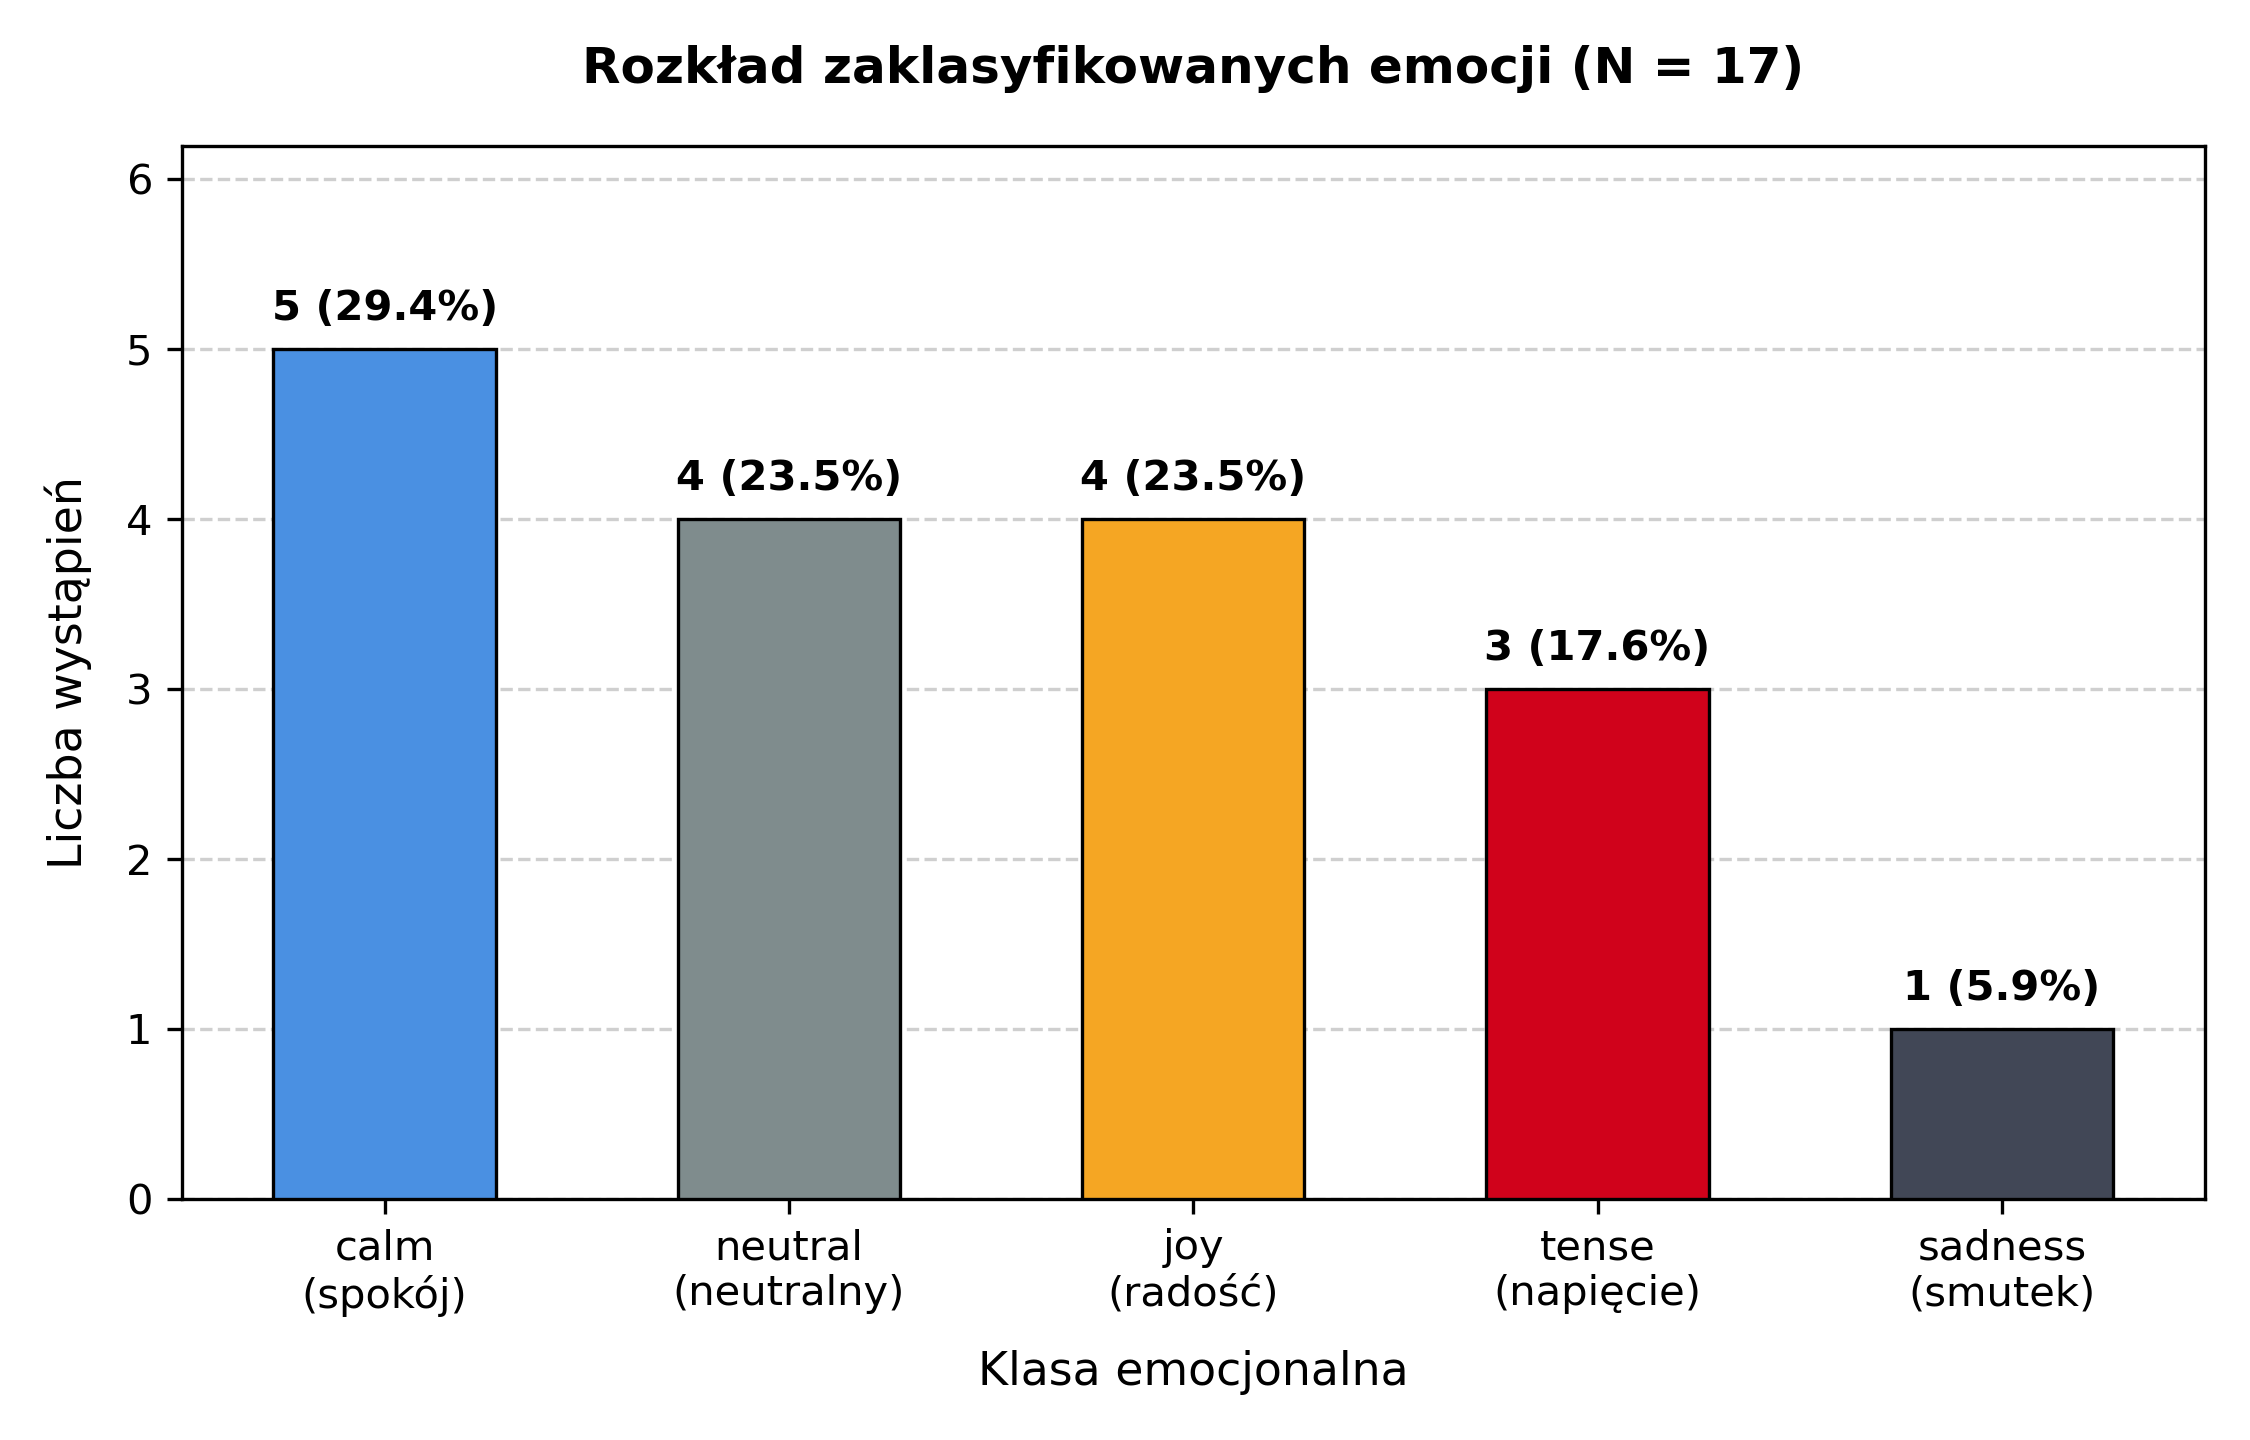
\includegraphics[width=0.7\linewidth]{figures/7/histogram_emocji.png}
        \caption{Przykład wyliczonych wartości dla przykładu z książki H. P. Lovecrafta}
        \label{fig:histogram}
    \end{figure}
    \FloatBarrier
    Do predykcji emocji następnie używany jest najpopularniejszy wynik (calm), jego 
    pewność (29\%), oraz margines od ostatniego najpopularniejszego (ok. 6 punktów procentowych).
\end{enumerate}

\subsubsection{Statystyczna agregacja i estymacja pewności}
Po sklasyfikowaniu wszystkich zdań w bieżącym oknie wyznaczany jest dyskretny rozkład 
prawdopodobieństwa wystąpienia poszczególnych nastrojów.
\begin{equation}
    P(k) = \frac{N_k}{N_{\text{total}}}
\end{equation}
gdzie $N_k$ oznacza liczbę zdań zakwalifikowanych do klasy $k$, natomiast $N_{\text{total}}$ to 
łączna liczba analizowanych zdań w oknie.

Ostateczna decyzja podejmowana jest w funkcji \textit{decide\_label} (listing~\ref{lst:decide_label}):
\begin{lstlisting}[style=pythonStyle, label={lst:decide_label}, caption={
    Wyznaczanie wiodącej etykiety, pewności oraz marginesu przewagi
}]
def decide_label(label_count: dict):
    ranked = sorted(label_count.items(), key=lambda x: x[1], reverse=True)
    top, p1 = ranked[0]
    p2 = ranked[1][1] if len(ranked) > 1 else 0.0
    return top, p1, round(p1 - p2, 4)
\end{lstlisting}

\section{Przykłady testów jednostkowych, integracyjnych i \textit{end-to-end}}
Dla poprawności działania systemu zastosowano testy jednostkowe oraz integracyjne we
wszytskich modułach oraz testy end-to-end (testy kompleksowe) w warstwie prezentacji.

\subsection{Warstwa serwisowa}
\begin{lstlisting}[style=pythonStyle, label={lst:backend_unit}, caption={
    Przykład testów jednostkowych w backendzie.
}]
def test_decide_label_multiple_with_margin():
    top, p1, margin = decide_label({"joy": 0.7, "sadness": 0.3})
    assert top == "joy"
    assert p1 == 0.7
    assert margin == 0.4

def test_decide_label_tie():
    top, p1, margin = decide_label({"joy": 0.5, "calm": 0.5})
    assert top in ("joy", "calm")
    assert p1 == 0.5
    assert margin == 0.0
\end{lstlisting}

\begin{lstlisting}[style=pythonStyle, label={lst:backend_integ}, caption={
    Przykład testów integracyjnych w backendzie.
}]
def test_upload_epub_success(client, session, monkeypatch):
    # Mock process_job background task to avoid executing external tools
    mock_called = []
    monkeypatch.setattr(
        "backend.src.routers.books.process_job",
        lambda job_id: mock_called.append(job_id)
    )

    dummy_epub = b"PK\x03\x04fake epub content"
    response = client.post(
        "/books/upload_epub",
        files={"file": ("my_novel.epub", io.BytesIO(dummy_epub), "application/epub+zip")}
    )
    assert response.status_code == 202
    data = response.json()
    assert "job_id" in data
    job_id = data["job_id"]

    # Verify database entry
    book = session.exec(select(Book).where(Book.job_id == job_id)).first()
    assert book is not None
    assert book.name == "my_novel.epub"
    assert book.status == "queued"
    assert book.browser_id == VALID_SID

    # Verify file saved on disk
    saved_file = job_dir(job_id) / "book.epub"
    assert saved_file.exists()
    assert saved_file.read_bytes() == dummy_epub
\end{lstlisting}

\subsection{Warstwa NLP}
\begin{lstlisting}[style=pythonStyle, label={lst:nlp_unit}, caption={
    Przykład testów jednostkowych w kontenerze NLP.
}]
def test_fit_model_space_median():
    predictor = VADPredictor()
    pred = np.array([
        [0.2, 0.4, 0.6],
        [0.4, 0.6, 0.8],
        [0.6, 0.8, 1.0],
    ])
    lex_ref = np.array(list(lexicon.values()))

    center, k = predictor.fit_model_space(pred, lex_ref)

    # Median of [0.2, 0.4, 0.6] is 0.4, etc.
    np.testing.assert_allclose(center, [0.4, 0.6, 0.8])
    assert len(k) == 3
\end{lstlisting}

\subsection{Warstwa prezentacji}
\begin{lstlisting}[style=pythonStyle, label={lst:frontend_unit}, caption={
    Przykład testów jednostkowych w warstwie prezentacji.
}]
describe('formatFileName', () => {
  it('returns empty string for empty input', () => {
    expect(formatFileName('')).toBe('');
  });

  it('formats simple hyphenated filename', () => {
    expect(formatFileName('my-book.epub')).toBe('My Book');
  });
\end{lstlisting}

\begin{lstlisting}[style=pythonStyle, label={lst:frontend_integ}, caption={
    Przykład testów integracyjnych dla warstwy prezentacji.
}]
describe('FileUpload', () => {
  beforeEach(() => {
    mockApi.mockReset();
  });

  it('renders "Choose EPUB file" label and a disabled Upload button initially', () => {
    render(<FileUpload onUploaded={vi.fn()} />);

    expect(screen.getByText('Choose EPUB file')).toBeInTheDocument();
    expect(screen.getByRole('button', { name: 'Upload' })).toBeDisabled();
  });
\end{lstlisting}

\begin{lstlisting}[style=pythonStyle, label={lst:frontend_integ}, caption={
    Przykład testów end-to-end dla warstwy prezentacji.
}]
test.describe.serial('Book Reader full-stack flow', () => {
  let page: Page;

  test.beforeAll(async ({ browser }) => {
    page = await browser.newPage();
    await waitForAppReady(page);
  }); 

  test.afterAll(async () => {
    await page?.close();
  });

  test('1. App loads and shows Book Reader heading', async () => {
    await expect(page.getByRole('heading', { name: 'Book Reader' })).toBeVisible();
    await expect(page.getByText('Upload an EPUB file to parse and read.')).toBeVisible();
    // Upload button is disabled without a file
    await expect(page.getByRole('button', { name: 'Upload' })).toBeDisabled();
  });
\end{lstlisting}
